\documentclass[12pt]{article}
\hyphenpenalty=10000
\usepackage[swedish]{babel}
\usepackage{amsmath}
\usepackage{graphicx}
\usepackage{float}

\title{Omfångsrikt problem: Mätning med märkning}
\author{Lukas Anderson}
\date{Maj 2023}

\begin{document}
\maketitle

\section*{Problemförklaring}
Ett företag ska designa en serie nya skålar. En av skålarna ska ha en cirkulär bottenyta med radien 7 cm och en cirkulär öppning med radien 12 cm. Skålens höjd ska vara 13 cm och dess ytterkant sedd från sidan ska kunna approximeras med kurvan $y=kx^2-m$ som visas i Figur 1.
\begin{figure}[h]
    \centering
    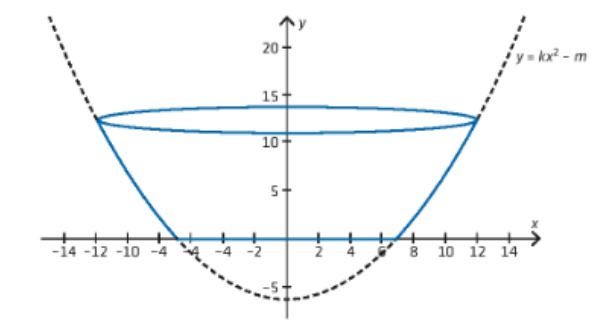
\includegraphics[width=\textwidth]{figur1.png}
    \caption{Skålens utseende}
\end{figure}
\subsection*{Uppgifter}
\begin{list}{-}{\leftmargin=1em\rightmargin=1em}
    \item Bestäm skålens volym med hjälp av {\it skivmetoden}.
    \item Designa två liknande skålar vars respektive volym är 3 liter.
    \item Eftersom skålarna är tänkta att användas vid bakning, så vill företaget att man på insidan av skålen ska kunna läsa av volymen. En av dina treliters-skålar ska ha sådana märkningar för varje liter. Bestäm på vilka höjder dessa märkningar ska sitta.
    \item Ta reda på hur man använder integraler för att beräkna volym med hjälp av {\it skalmetoden}. Redogör för hur metoden fungerar och lista ut hur du kan använda den för att beräkna volymen av någon av skålarna ovan. Beräkna också den volymen.
    \item Du behärskar nu två olika metoder för att beräkna volymen av en rotationskropp: {\it skivmetoden\/} och {\it skalmetoden}. Diskutera metodernas för- och nackdelar.
\end{list}
\section*{Uppgift 1}
\subsection*{Bestäm skålens volym med hjälp av {\it skivmetoden}.}
Formeln för skivmetoden är $V=\pi\int_{0}^{13}{g(y)}^2dy$
Där funktionen $g(y)$ är $f(x)$ uttryckt som en funktion av $y$.
\\\\
För att finna $g(y)$ identifierar vi först funktionen $f(x)=y$ som beskriver skålens form och kan beskrivas som $y=kx^2-m$. Att skålen har radien 7 cm innebär att $f(x)$ har rötterna $(7,0) (-7,0)$
För att finna $k$ och $m$ löser ställer vi upp följande ekvation:\\
\begin{align*}
    kx^2-m&=k(x-7)(x+7)\\
    kx^2-m&=k(x^2-49)\\
    kx^2-m&=kx^2-49k\\
    m&=49k\\
\end{align*}
Vilket ger oss att $m=49k$ och att $f(x)=y=kx^2-49k$.
\\\\
För att finna $k$ löser vi följande ekvation:
\begin{align*}
    f(12)=13\\
    13&=k{(12)}^2-49k\\
    13&=144k-49k\\
    13&=95k\\
    k&=\frac{13}{95}\\
\end{align*}
Vilket ger oss att $k=\frac{13}{95}$ och att $f(x)=y=\frac{13}{95}x^2-\frac{637}{95}$.
\\\\
Detta visas i Figur 2.
\begin{figure}[h]
    \centering
    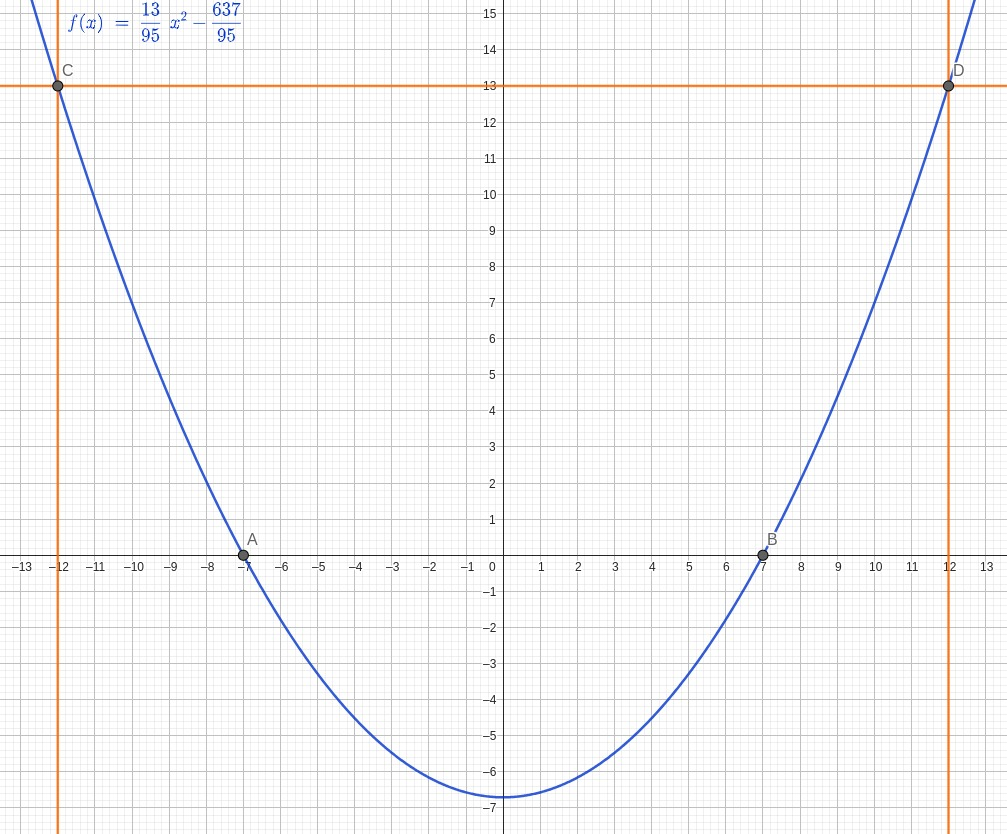
\includegraphics[width=0.8\textwidth]{figur2.jpg}
    \caption{Skålens utseende med $f(x)$ uttryckt som en funktion}
\end{figure}
\newpage
Med $f(x)=\frac{13}{95}x^2-\frac{637}{95}$ kan vi räkna ut $g{(y)}^2$ då $g(y)=x$ och $f(x)=y$:
\begin{align*}
    \frac{13}{95}x^2-\frac{637}{95}&=y\\
    \frac{13}{95}x^2&=y+\frac{637}{95}\\
    x^2&=\frac{y+\frac{637}{95}}{\frac{13}{95}}\\
    g{(y)}^2&=\frac{y+\frac{637}{95}}{\frac{13}{95}}\\
    g{(y)}^2&=\frac{95y+637}{13}\\
\end{align*}
Detta ger oss att $g{(y)}^2=\frac{95y+637}{13}$.
För att räkna ut volymen med formeln $V=\pi\int_{0}^{13}{g(y)}^2dy$ måste vi först bestämma den primitiva funktionen $H(y)$ till funktionen $h(y)=g{(y)}^2=\frac{95y+637}{13}$.
\begin{align*}
    h(y)&=\frac{95y+637}{13}\\
    h(y)&=\frac{95}{13}y+\frac{637}{13} \Rightarrow H(y)=\frac{95/13}{2}y^2+\frac{637}{13}y+C\\
    H(y)&=\frac{95}{26}y^2+\frac{637}{13}y+C\\
\end{align*}
Detta ger oss att $H(y)=\frac{95}{26}y^2+\frac{637}{13}y+C$.
\newpage
Vi kan nu skriva om formeln $V=\pi\int_{0}^{13}{g(y)}^2dy$:
\begin{align*}
    V&=\pi\int_{0}^{13}{g(y)}^2dy\\
    V&=\pi\int_{0}^{13}{h(y)}dy\\
    V&=\pi\int_{0}^{13}{h(y)}dy\Rightarrow V=\pi{\left[{H(y)}\right]}_{0}^{13}\\
    V=\pi{\left[{H(y)}\right]}_{0}^{13}&=\pi\left(\frac{95}{26}{(13)}^2+\frac{637}{13}(13)-\frac{95}{26}{(0)}^2-\frac{637}{13}(0)\right)\\
    V&=\pi\left(\frac{95}{26}{(13)}^2+\frac{637}{13}(13)\right)\\
    V&=\pi\left(\frac{95}{26}{(169)}+\frac{637}{13}(13)\right)\\
    V&=\pi\left(\frac{16055}{26}+\frac{8271}{13}\right)\\
    V&=\frac{16055\pi}{26}+\frac{8271\pi}{13}\\
    V&\approx 3938.7\text{ cm}^3\\
\end{align*}
Skivmetoden ger oss att skålen har volymen $V\approx 3938.7\text{ cm}^3$.
\newpage
\section*{Uppgift 2}
\subsection*{Designa två liknande skålar vars respektive volym är 3 liter.}
För att designa två liknande skålar vars respektive volym är 3 liter börjar med att bestämma radien av skålens bottenyta. För den första skålen Skål 1, bestämmer jag att radien ska vara 4 cm. För den andra skålen Skål 2, bestämmer jag att radiens ska vara 6 cm.
\subsection*{Skål 1:}
För att bestämma skålens form börjar jag med att bestämma funktionen $f(x)$ som beskriver skålens form. Jag bestämmer att skålen ska ha en bottenyta med radien 4 cm. Detta innebär att $f(x)$ har rötterna $(4,0) (-4,0)$ och att $f(x)=k(x-4)(x+4)$. $k$ i funktionen bestämmer hur aggresiv lutningen är på skålens sidor. Sambandet mellan $k$ och skålens form visas i Figur 3a och 3b.\\
\begin{figure}[H]
    \centering
    \renewcommand{\thefigure}{3a}
    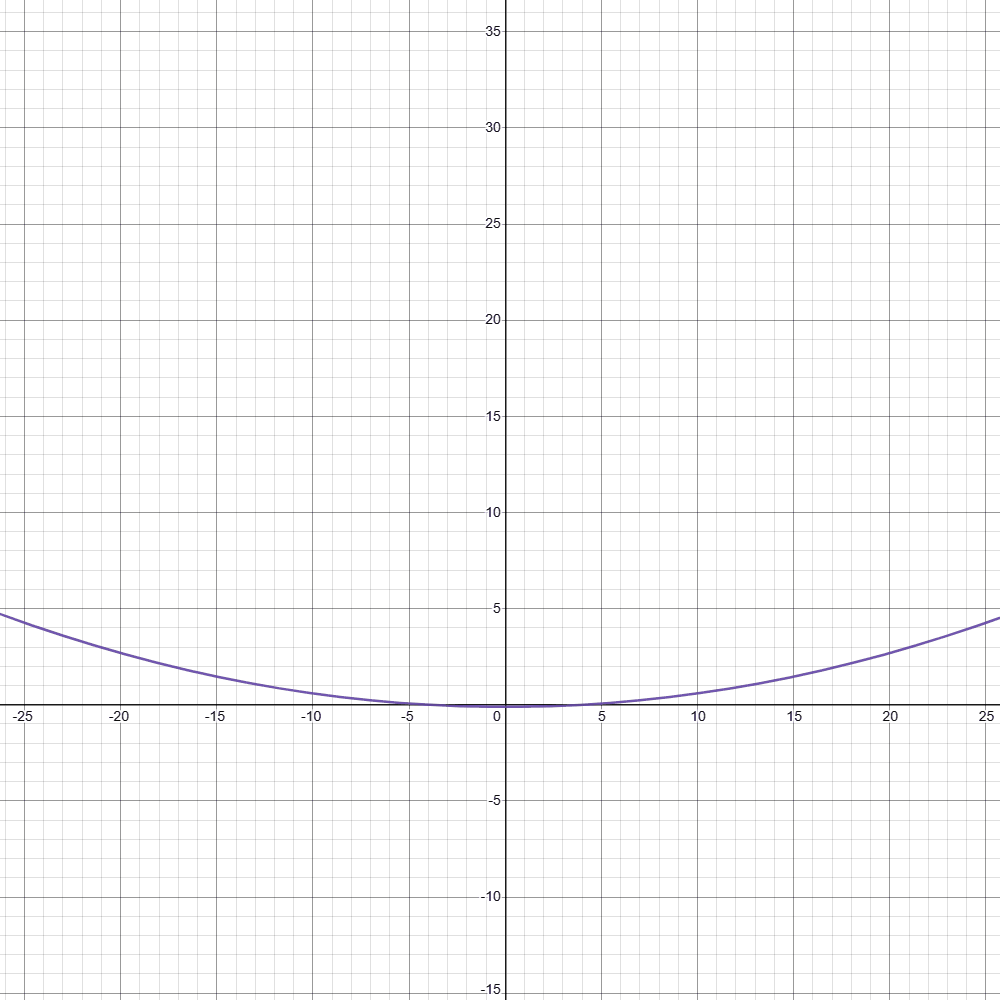
\includegraphics[width=0.6\textwidth]{figur3a.png}
    \caption{Skålens form uttrycky som $f(x)$ då $k$ går från $0.01$ till $0.3$.}
\end{figure}
\begin{figure}[H]
    \centering
    \renewcommand{\thefigure}{3b}
    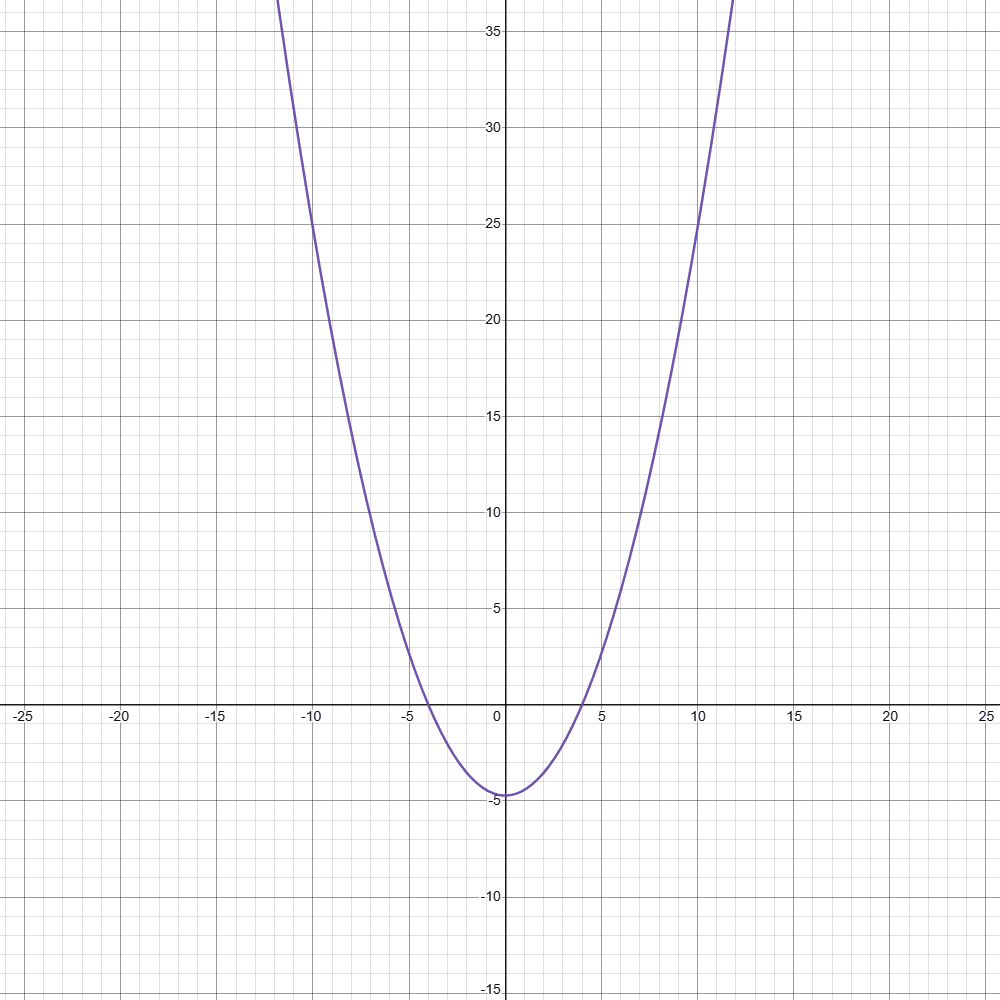
\includegraphics[width=0.6\textwidth]{figur3b.png}
    \caption{Skålens form uttrycky som $f(x)$ då $k$ går från $0.01$ till $0.3$.}
\end{figure}
Jag bestämmer att $k=0.1$ vilket ger $f(x)=0.1(x-4)(x+4)$.
\\\\
Funktionen $f(x)$ kan då skrivas i formen $kx^2-m$:
\begin{align*}
    f(x)&=0.1(x-4)(x+4)\\
    f(x)&=0.1(x^2-16)\\
    f(x)&=0.1x^2-1.6\\
\end{align*}
\\
Detta ger oss att $f(x)=0.1x^2-1.6$ som visas i Figur 4.
\begin{figure}[H]
    \centering
    \renewcommand{\thefigure}{4}
    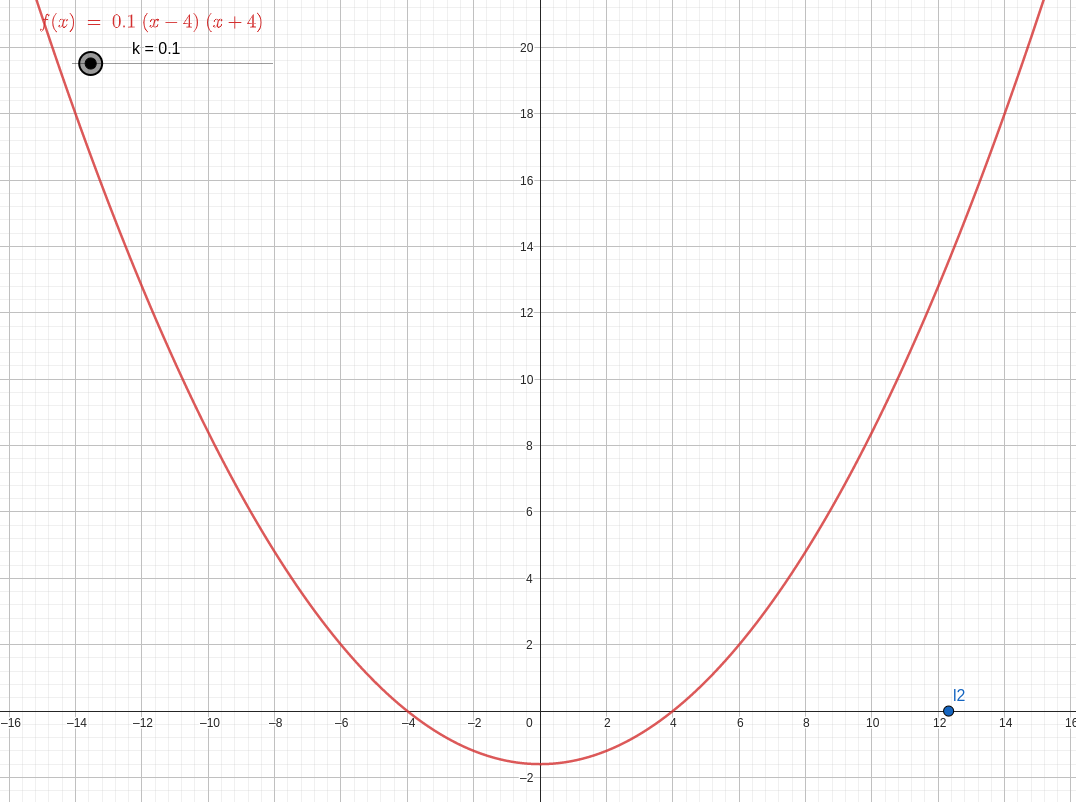
\includegraphics[width=0.8\textwidth]{figur4.png}
    \caption{Skålens utseende med $f(x)$ uttryckt som en funktion}
\end{figure}
Då vi har funktionen $f(x)$ kan vi räkna ut $g{(y)}^2$ då $g(y)=x$ och $f(x)=y$:
\begin{align*}
    0.1x^2-1.6&=y\\
    0.1x^2&=y+1.6\\
    x^2&=\frac{y+1.6}{0.1}\\
    g{(y)}^2&=\frac{y+1.6}{0.1}\\
    g{(y)}^2&=10y+16\\
\end{align*}
Detta ger oss att $g{(y)}^2=10y+16$.
Vi bestämmer att funktionen $h(y)=g{(y)}^2$ och söker nu den primitiva funktionen $H(y)$ till $h(y)$. Vi finner $H(y)$:
\begin{align*}
    h(y)&=10y+16 \Rightarrow H(y)=5y^2+16y+C\\
    H(y)&=5y^2+16y+C\\
\end{align*}
Detta ger oss att $H(y)=5y^2+16y+C$.\\
Vi kan nu skriva om formeln $V=\pi\int_{0}^{l}{g(y)}^2dy$ där $l$ är skålens höjd och volymen $V$ är $3000$ cm$^3$:
\begin{align*}
    V&=\pi\int_{0}^{l}{g(y)}^2dy\\
    3000&=\pi\int_{0}^{l}{h(y)}dy\\
    3000&=\pi\int_{0}^{l}{h(y)}dy\Rightarrow 3000=\pi{\left[{H(y)}\right]}_{0}^{l}\\
    3000&=\pi\left(5{l}^2+16l-5{(0)}^2-16(0)\right)\\
    3000&=\pi\left(5{l}^2+16l\right)\\
\end{align*}
Detta ger oss andragradsekvationen $3000=\pi\left(5{l}^2+16l\right)$. Denna löser vi för $l$ med hjälp av PQ-formeln:
\begin{align*}
    3000&=\pi\left(5{l}^2+16l\right)\\
    0&=5\pi{l}^2+16\pi{l}-3000\\
    0&=5{l}^2+16{l}-\frac{3000}{\pi}\\
    0&=l^2+\frac{16}{5}l-\frac{3000}{\pi5}\\
    0&=l^2+\frac{16}{5}l-\frac{600}{\pi}\\
    l&=-\frac{\frac{16}{5}}{2}\pm\sqrt{{\left(\frac{\frac{16}{5}}{2}\right)}^2+\left(\frac{600}{\pi}\right)}\\
    l&=-\frac{8}{5}\pm\sqrt{{\left(\frac{8}{5}\right)}^2+\left(\frac{600}{\pi}\right)}\\
    l&=-\frac{8}{5}\pm\sqrt{\frac{64\pi+15000}{25\pi}}\\
    l_1&\approx 12.3\text{ cm}\\
    l_2&\approx -15.5\text{ cm}\\
\end{align*}
Detta ger att $l_1\approx 12.3\text{ cm}$ och $l_2\approx -15.5\text{ cm}$.
Då $l$ är skålens höjd kan vi förkasta $l_2$ då den är negativ. Detta ger oss att höjden $l\approx 12.3\text{ cm}$.\\
Skål 1 har då en bottenyta med radien 4 cm, en höjd på 12.3 cm samt en volym på 3 liter.
\subsection*{Skål 2:}
Vi följer samma process för denna skål. Vi börjar med att bestämma att bottenytan har en radie på 8 cm. Detta ger oss att $f(x)$ har rötterna $(8,0) (-8,0)$ och att $f(x)=k(x-8)(x+8)$. $k$ bestämmer vi är 0.2 vilket ger $f(x)=0.2(x-8)(x+8)$. Denna funktion kan skrivas om till $f(x)=0.2x^2-\frac{64}{5}$ som visas i Figur 5.
\begin{figure}[H]
    \centering
    \renewcommand{\thefigure}{5}
    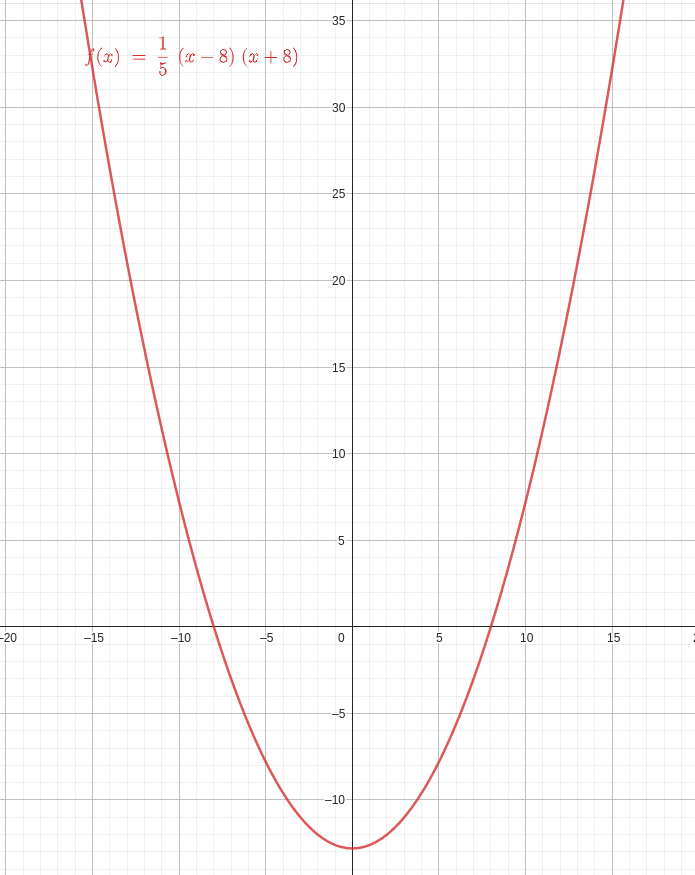
\includegraphics[width=0.7\textwidth]{figur5.png}
    \caption{Formen av Skål 2 uttryckt som en funktion $f(x)$}
\end{figure}
Vi kan nu räkna ut $g{(y)}^2$ då $g(y)=x$ och $f(x)=y$:
\begin{align*}
    0.2x^2-\frac{64}{5}&=y\\
    0.2x^2&=y+\frac{64}{5}\\
    x^2&=\frac{y+\frac{64}{5}}{\frac{1}{5}}\\
    g{(y)}^2&=\frac{y+\frac{64}{5}}{\frac{1}{5}}\\
    g{(y)}^2&=5y+64\\
\end{align*}
Detta ger oss att $g{(y)}^2=5y+64$.
Vi bestämmer att funktionen $h(y)=g{(y)}^2$ och söker nu den primitiva funktionen $H(y)$ till $h(y)$. Vi finner $H(y)$:
\begin{align*}
    h(y)&=5y+64 \Rightarrow H(y)=\frac{5}{2}y^2+64y+C\\
    H(y)&=\frac{5}{2}y^2+64y+C\\
\end{align*}
Detta ger oss att $H(y)=\frac{5}{2}y^2+64y+C$.
\newpage
Vi kan nu skriva om formeln $V=\pi\int_{0}^{l}{g(y)}^2dy$ där $l$ är skålens höjd och den övre integrationsgränsen och volymen $V$ är $3000$ cm$^3$:
\begin{align*}
    V&=\pi\int_{0}^{l}{g(y)}^2dy\\
    3000&=\pi\int_{0}^{l}{h(y)}dy\\
    3000&=\pi\int_{0}^{l}{h(y)}dy\Rightarrow 3000=\pi{\left[{H(y)}\right]}_{0}^{l}\\
    3000&=\pi\left(\frac{5}{2}{l}^2+64l-\frac{5}{2}{(0)}^2-64(0)\right)\\
    3000&=\pi\left(\frac{5}{2}{l}^2+64l\right)\\
    3000&=\pi\frac{5}{2}l^2+64\pi l\\
    0&=\pi\frac{5}{2}l^2+64\pi l-3000\\
    0&=\frac{5}{2}l^2+64l-\frac{3000}{\pi}\\
    0&=l^2+\frac{128}{5}l-\frac{1200}{\pi}\\
    l&=-\frac{\frac{128}{5}}{2}\pm\sqrt{{\left(\frac{\frac{128}{5}}{2}\right)}^2+\left(\frac{1200}{\pi}\right)}\\
    l&=-\frac{64}{5}\pm\sqrt{{\left(\frac{64}{5}\right)}^2+\left(\frac{1200}{\pi}\right)}\\
    l&=-\frac{64}{5}\pm\sqrt{\frac{4096\pi+30000}{25\pi}}\\
    l_1&\approx 10.6\text{ cm}\\
    l_2&\approx -36.2\text{ cm}\\
\end{align*}
Detta ger att $l_1\approx 10.6\text{ cm}$ och $l_2\approx -36.2\text{ cm}$. Än en gång ignorerar vi den negativa lösningen då skålens höjd ej kan vara negativ. Detta ger oss att höjden $l\approx 10.6\text{ cm}$. Skål 2 har då en bottenyta med radien 8 cm, en höjd på 10.6 cm samt en volym på 3 liter.
\newpage
\section*{Uppgift 3}
\subsection*{Märkning av volym}
Då skålarna vi designat ska användas vid bakning måste det finnas en gradering av volym på insidan av skålarna. I detta fall använder vi Skål 2 som exempel. För att beräkna var dessa graderingar ska sitta använder vi samma metod som vi använde då vi sökte höjden av Skål 2. Vi börjar med att ställa upp ekvationen för volymen vid den första markeringen, 1 liter, $V=1000$ då vi än en gång söker höjden $l$ som är den övre integrationsgränsen:
\begin{align*}
    V&=\pi\int_{0}^{l}{g(y)}^2dy\\
    1000&=\pi\int_{0}^{l}{h(y)}dy\\
    1000&=\pi\int_{0}^{l}{h(y)}dy\Rightarrow 3000=\pi{\left[{H(y)}\right]}_{0}^{l}\\
    1000&=\pi\left(\frac{5}{2}{l}^2+64l-\frac{5}{2}{(0)}^2-64(0)\right)\\
    1000&=\pi\left(\frac{5}{2}{l}^2+64l\right)\\
    1000&=\pi\frac{5}{2}l^2+64\pi l\\
    0&=\pi\frac{5}{2}l^2+64\pi l-1000\\
    0&=\frac{5}{2}l^2+64l-\frac{1000}{\pi}\\
    0&=l^2+\frac{128}{5}l-\frac{2000}{\pi}\\
    l&=-\frac{\frac{128}{5}}{2}\pm\sqrt{{\left(\frac{\frac{128}{5}}{2}\right)}^2+\left(\frac{2000}{\pi}\right)}\\
    l_1&=4.3\text{ cm}\\
    l_2&=-29.9\text{ cm}\\
\end{align*}
\newpage
Detta ger oss att $l_1=4.3\text{ cm}$ och $l_2=-29.9\text{ cm}$. Vi förkastar återigen den negativa lösningen då höjden ej kan vara negativ. Detta ger oss att höjden av den första markeringen, 1 liter, är $l=4.3\text{ cm}$.
\\\\
Vi upprepar processen för att finna höjden av den andra markeringen, 2 liter, vilket ger höjden $l=7.7\text{ cm}$.\\
\section*{Uppgift 4}
\subsection*{Vad är skalmetoden och hur används den för att beräkna volymen av en reotationskropp?}
Skalmetoden är en metod för att beräkna volymen av en rotationskropp genom att dela upp kroppen i tunna cylinderformade skal. Dessa skal har en tjocklek $\Delta x$, radien $x_i$ och en höjd $f(x_i)$ där $f(x_i)$ är en funktion som beskriver formen av kroppen och där $x_i$ är integrationsvariabeln. Detta visas i Figur 6.
\begin{figure}[H]
    \centering
    \renewcommand{\thefigure}{6}
    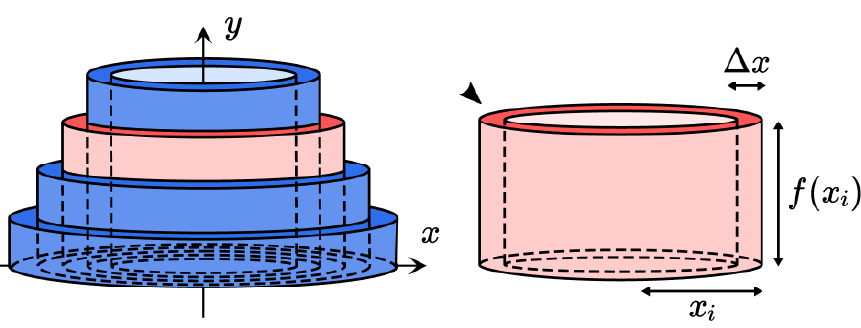
\includegraphics[width=\textwidth]{figur6.png}
    \caption{Demonstration av skalmetoden}
\end{figure}
Om man vecklar ut ett av dessa skal till ett rätblock får rätblocket volymen $V_i=2\pi x_i\cdot f(x_i)\cdot \Delta x$. Detta visas i Figur 7.
\newpage
\begin{figure}[H]
    \centering
    \renewcommand{\thefigure}{7}
    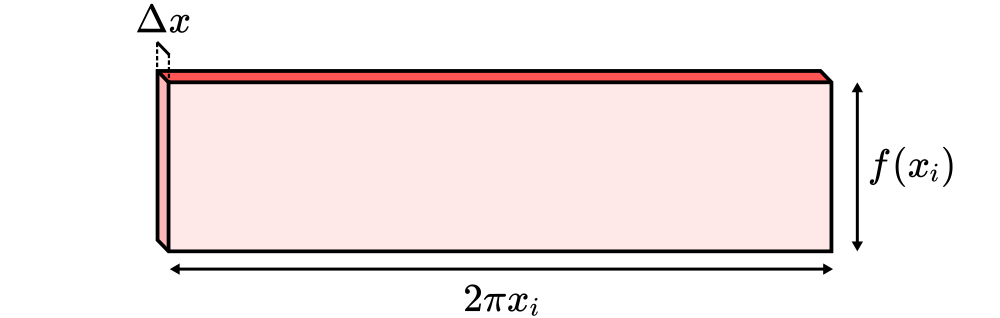
\includegraphics[width=\textwidth]{figur7.png}
    \caption{Demonstration av skalmetoden}
\end{figure}
För att uppnå en högre noggrannhet i beräkningen av\\
rotationskroppens volym låter vi istället $\Delta x$ gå mot 0 medan antalet skal går mot oändligheten och summerar volymen av alla skal. Detta ger oss att volymen $V$ av 
rotationskroppen är:
\begin{align*}
    V&=\int_{a}^{b}2\pi x\cdot f(x) dx\\
    V&=2\pi\int_{a}^{b}x\cdot f(x) dx\\
\end{align*}
I integralen är integrationsgränserna a och b de två punkter där rotationskroppen börjar och slutar i x-led då kroppen roteras runt y-axeln.\\
\subsection*{Beräkna volymen av Skål 2 med skalmetoden:}
Funktionen som beskriver formen av Skål 2 är $f(x)=0.2x^2-\frac{64}{5}$. Då formeln för skalmetoden beräknar volymen mellan funktionen och x-axeln måste vi utesluta den del av funktionen som är under x-axeln. Detta gör vi genom att sätta integrationsgränserna till $a=8$ och b till den punkt där funktionen ger höjden av skålen $f(x)=10.6$. Vi adderar sedan volymen av en cylinder med radien 8 cm och höjden 10.6 cm för att få volymen av hela skålen. Grafen samt beräkningen av de två volymerna visas i Figur 8.
\begin{figure}[H]
    \centering
    \renewcommand{\thefigure}{8}
    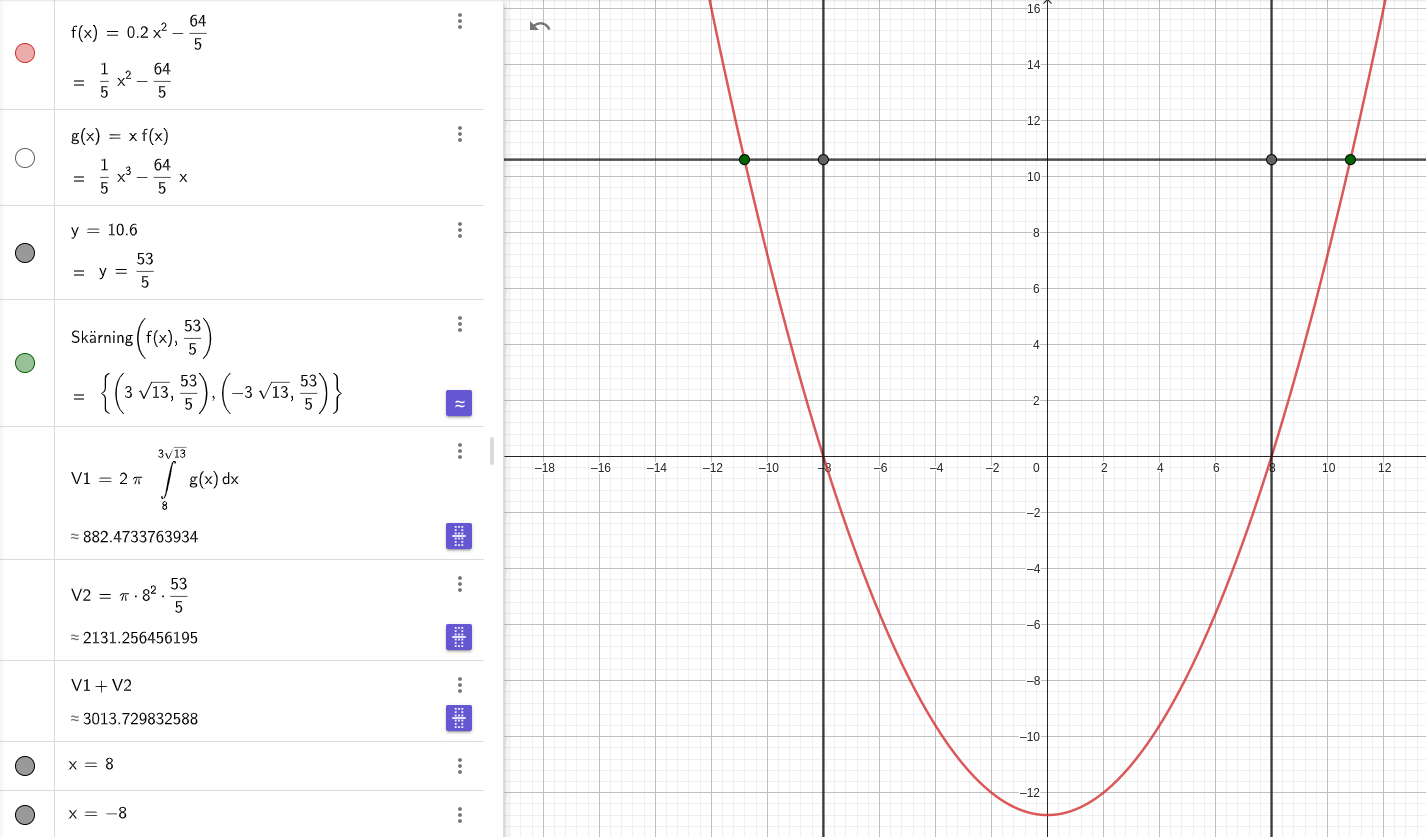
\includegraphics[width=\textwidth]{figur8.png}
    \caption{Demonstration av skalmetoden}
\end{figure}
Vi beräknar volymen av skålen med skalmetoden:\\
\begin{align*}
    V&=V_{cylinder}+V_{skal}\\
    V_{cylinder}&=\pi 8^2\cdot 10.6\\
    V_{cylinder}&=\frac{3392}{5}\pi\\
    \\
\end{align*}
Vi finner den övre integrationsgränsen:
\begin{align*}
    f(x)=10.6&\Rightarrow x=3\sqrt{13}
\end{align*}
Vi beräknar volymen av skålen från $x=8$ till $x=3\sqrt{13}$ med skalmetoden:
\begin{align*}
    V_{skal}&=\int_{8}^{3\sqrt{13}}2\pi x\cdot f(x) dx\\
    V_{skal}&=2\pi\int_{8}^{3\sqrt{13}}x\cdot f(x) dx\\
    V_{skal}&=2\pi\int_{8}^{3\sqrt{13}}x\cdot (0.2x^2-\frac{64}{5}) dx\\
    V_{skal}&=2\pi\int_{8}^{3\sqrt{13}}0.2x^3-\frac{64}{5}x dx\\
    V_{skal}&=2\pi{\left(\frac{0.2}{4}x^4-\frac{64}{10}x^2\right)}_{8}^{3\sqrt{13}}\\
    V_{skal}&=2\pi\left(\frac{0.2}{4}{(3\sqrt{13})}^4-\frac{64}{10}{(3\sqrt{13})}^2-\frac{0.2}{4}{(8)}^4+\frac{64}{10}{(8)}^2\right)\\
    V_{skal}&=2\pi\left(\frac{0.2}{4}{(3\sqrt{13})}^4-\frac{64}{10}{(3\sqrt{13})}^2-\frac{0.2}{4}{(8)}^4+\frac{64}{10}{(8)}^2\right)\\
    \\
    V&=V_{cylinder}+V_{skal}\\
    V&=3013.8 \text { cm}^3\\
\end{align*}
Detta ger oss att $V\approx 3013.8 \text { cm}^3$ vilket stämmer med de beräkningar som gjordes med skivmetoden.
\newpage
\section*{Uppgift 5}
\subsection*{Diskutera skalmetoden och skivmetoden}
Både skal- och skivmetoden är två metoder för att beräkna volymen av en rotationskropp. Båda metoderna fungerar genom att dela upp kroppen i mindre delar och sedan summera volymen av dessa delar. Skivmetoden delar upp kroppen i skivor med tjockleken $\Delta y$ medan skalmetoden delar upp kroppen i skal med tjockleken $\Delta x$. De båda metoderna kan anpassas för att för att beräkna rotationer runt både x- och y-axeln. Därför är metodernas användbarhet lika stor men det finns vissa skillnader mellan metoderna. Då skalmetoden tillåter rotation runt y-axeln utan att behöva anpassa om en funktion som $f(x)=y$ till att bli en funktion $f(y)=x$ är skalmetoden mer användbar för att beräkna volymen av en rotationskropp runt y-axeln. Skivmetoden är dock mer användbar för att beräkna volymen av en\\ rotationskropp runt x-axeln då den inte kräver någon anpassning av funktionen $f(x)=y$ till $f(y)=x$. På detta sätt är dessa metoder varandras inverser och komplementerar varandra. Det är därför användbart att kunna båda metoderna för att uppnå maximal effektivitet vid beräkningar av volymer av rotationskroppar, oavsett vilken axel de roterar runt.

\subsection*{Utvärdering av resultat}
Då båda metoderna gav samma resultat för volymen av Skål 2 kan vi anta att resultatet är korrekt. Sammma metod som användes för att beräkna volymen av Skål 2 användes för att beräkna volymen av Skål 1. Då denna metod blivit bekräftas av de båda beräkningarna av Skål 2:s volym är beräkningarna pålitliga.

\subsection*{Tillämpningar}
Det senario som ställs fram i uppgiften är ett av de många tillämplingarna av dessa metoder i verkligheten. Då varje skål, glas och behållare i världen måste designas för att kunna produceras med lämpliga dimensioner är dessa metoder användbara för att beräkna volymen av dessa behållare. Dessa metoder är även användbara inom utvecklingen av datorgrafik och skapandet av digitala tredimensionella objekt då dessa objekt kan beskrivas med\\ funktioner som kan användas för att beräkna volymen och formen av en dator.

\subsection*{Förbättringar}
En förbättring av arbetet hade varit att göra designen av Skål 1 och Skål 2 mer realistiskt genom att ta hänsyn till skålarnas syfte och det fortsatta arbetet med dem under det första steget av designen. Exempelvis hade en skål för bakning som skall kunna mäta volymer upp till 3 liter i verkligheten haft en större volym än 3 liter då en märkning för mätning ej går att placeras på skålens kant. Detta hade lett till att skålarna hade fått en mer realistisk form och volym.
\end{document}